\documentclass[11pt,french]{article} % police taille 11 car 10 c'est pour les terroristes
\usepackage{babel} % paquet qui permet de gérer les différentes langues
\usepackage{graphicx} % paquet pour inclure des images
\usepackage{float}
\usepackage{titling}
\usepackage{environ}
\usepackage{amsmath,amsfonts,amssymb,amsthm}
\usepackage{geometry}
\geometry{legalpaper, margin=100pt}

\setlength{\parindent}{0pt}

\NewEnviron{NORMAL}{% environnement used to scale math equations 
    \scalebox{1.2}{$\BODY$} 
} 

\begin{document}

\begin{figure}[t]
    \centering
		\advance\leftskip-0.2cm
    
\includegraphics[width=8cm]{inp_n7.png} % joli logo de l'N7
\end{figure}

\title{\vspace{0.5cm} \textbf{Rapport de bureau d'études\\Automatique Systèmes Cyber Physique}} 
\author{RAGOT Cyrian}
\renewcommand{\maketitlehookc}{%
	\vspace{3cm}
  \begin{center}
		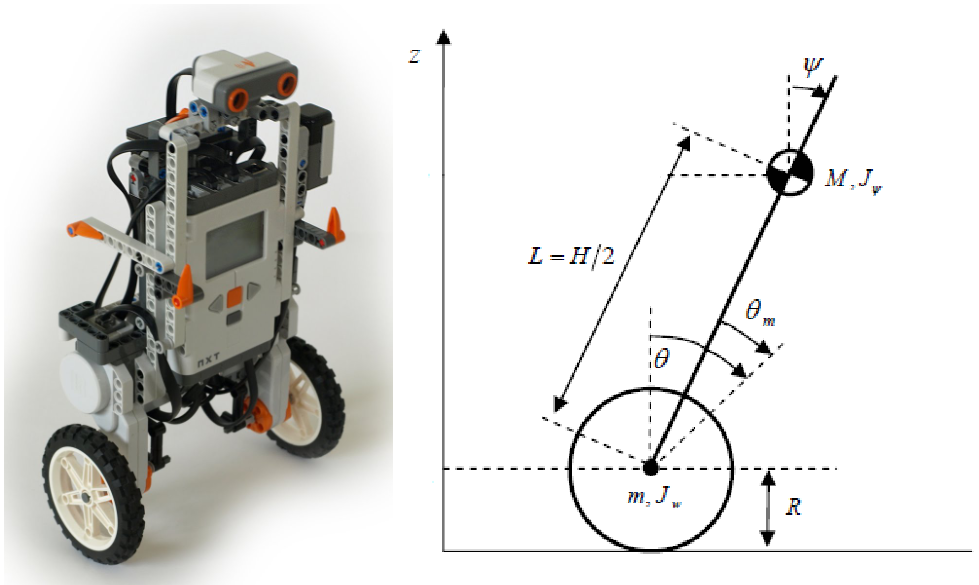
\includegraphics[width=14cm]{segway.png} % image segway 1ere page
  \end{center}
}
\date{\vspace{1cm}\vfill Département Sciences du Numérique - Première année \\
2023-2024 }

\maketitle

\newpage % génère un saut de page, en gros retour à la ligne mais pour une page
\tableofcontents % génère un sommaire des sections du document
\newpage

\section{Introduction}


\newpage
\section{Modèle du pendule inversé}

Dans cette partie, nous étudierons un modèle simple d'un pendule inversé contrôlé par retour d'état. Le système contrôlé issu des équations physiques de la dynamique est \\


\begin{equation}
	\NORMAL{
  \left\{
    \begin{array}{l}
			\dot{x}_1(t) = x_2(t) \\
			\dot{x}_2(t) = \frac{g}{l}sin(x_1(t))-\frac{cos(x_1(t))u(t)}{l} \\
			\dot{x}_1(0) = x_{0,1} = \alpha_0 \\
			\dot{x}_2(0) = x_{0,2} = \dot\alpha_0, \\
    \end{array}
  \right.
	}
\end{equation}

avec

\begin{description}
	\item[--] $\mathbf{g = 9.81 m/s^2}$ constante de gravité
	\item[--] $\mathbf{l = 10 m}$ longueur du pendule
	\item[--] $\mathbf{t_0 = 0 s}$ instant initial
	\item[--] $\boldsymbol{x(t) = (x_1(t), x_2(t))^\intercal = (\alpha(t), \dot\alpha(t))^\intercal}$ variable d'état 
	\item[--] $\boldsymbol{(x_e,u_e)^\intercal = (0,0,0)^\intercal}$ point de fonctionnement
	\item[--] $\boldsymbol{u(t)}$ contrôle par retour d'état
\end{description}

% TODO figure du pendule avec alpha

On souhaite stabiliser le système à l'origine (la position verticale du pendule inversé), cependant le système non contrôlé n'est pas stable à l'origine. En effet,  \\


On choisit alors un contrôle par retour d'état linéaire $u(t) = u_e + K(x(t) - x_e)$ avec $K = (k_1, k_2)$.





\newpage
\section{Modèle du robot Lego}

\newpage
\section{Robot Lego NXT}

\newpage
\section{Conclusion}


\end{document}
